%!TEX root=../../main.tex

\chapter{Multiple linear regression}
\label{multipleLinearRegression}
\index{multiple linear regression|textbf}

In most practical settings, more than one explanatory variable is likely to be associated with a response. This chapter discusses how the ideas behind simple linear regression can be extended to a model with multiple predictor variables. 

There are many applications of multiple regression; one of the more important is the use of multiple regression to estimate an association while adjusting for possible confounding variables. Confounding was introduced in Chapter~\ref{introductionToData} and further explored in a case study in Section~\ref{exploratoryDataAnalysis}, where age was found to be a confounder for the association between ethnicity and the amount of financial support from the State of California. Sections~\ref{introductionMultipleLinearRegression} and \ref{simpleVsMultipleRegression} present a new example where an apparent association between a response and predictor may be distorted by a confounder, and show how multiple regression can directly summarize the relationship between several potentially associated variables.

Section~\ref{modelSelectionPrediction} discusses another application of multiple regression\textemdash constructing a prediction model that effectively explains the observed variation in the response variable. In this setting, the goal is to make accurate predictions for the response variable, given information specified by the predictor variables in the model.

The other sections in the chapter outline general principles of multiple regression, including the statistical model, methods for assessing quality of model fit, categorical predictors with more than two levels, interaction, and the connection between ANOVA and regression.

\begin{comment}

Simple linear regression is useful when the main interest of a study is the association of a response variable with a single predictor or explanatory variable.  Scientific investigations are rarely that simple, however; in most settings more than one explanatory variable is likely to be associated with a response, and multiple linear regression can be important model in those situations.  The study of risk factors for cognitive decline in adults outlined in the next section is one of those situations.

Section~\ref{introductionMultipleLinearRegression} discusses the concept of confounding, when the apparent association between a response and a primary predictor might be distorted when a third variable associated with both the response and the predictor is ignored.  In the example used, the response variable is a measure of cognitive decline (\var{RFFT} in the PREVEND data), the primary predictor of interest is the use of a drug to lower cholesterol and the possible confounder is age. 

Sections~\ref{simpleVsMultipleRegression} shows how multiple regression can be used to estimate the association between RFFT and statin use, after adjusting for age.  Adjusting for one or more possible confounders is not the only application of multiple regression, but it is one of the more important.   The model used is a simple model with two predictors but it illustrates many of the important ideas in multiple regression; it is a good way to start the study of more complicated models and other applications.

Section~\ref{Evaluating the fit of a multiple regression model} continues with a model with two predictors, showing methods for evaluating the quality of the fit of the model. Section~\ref{generalMultipleRegression} then outlines the general ideas of multiple regression.  Additional applications of multiple regression are illustrated in the last three sections of the chapter.

\end{comment}

\section{Introduction to multiple linear regression}
\label{introductionMultipleLinearRegression}

Statins are a class of drugs widely used to lower cholesterol. There are two main types of cholesterol: low density lipoprotein (LDL) and high density lipoprotein (HDL).\footnote{Total cholesterol level is the sum of LDL and HDL levels.} Research suggests that adults with elevated LDL may be at risk for adverse cardiovascular events such as a heart attack or stroke. In 2013, a panel of experts commissioned by the American College of Cardiology and the American Heart Association recommended that statin therapy be considered in individuals who either have any form of atherosclerotic cardiovascular disease\footnote{i.e., arteries thickening and hardening with plaque} or have LDL cholesterol levels $\geq 190$ mg/dL, individuals with Type II diabetes ages 40 to 75 with LDL between 70 to 189 mg/dL, and non-diabetic individuals ages of 40 to 75 with a predicted probability of future clogged arteries of at least 0.075.\footnote{Circulation. 2014;129:S1-S45. DOI: 10.1161/01.cir.0000437738.63853.7a}

Some health policy analysts have estimated that if the new guidelines were to be followed, almost half of Americans ages 40 to 75 and nearly all men over 60 would be prescribed a statin. However, some physicians have raised the question of whether treatment with a statin might be associated with an increased risk of cognitive decline.\footnote{Muldoon, Matthew F., et al. Randomized trial of the effects of simvastatin on cognitive functioning in hypercholesterolemic adults. The American journal of medicine 117.11 (2004): 823-829.}\textsuperscript{,}\footnote{King, Deborah S., et al. Cognitive impairment associated with atorvastatin and simvastatin. Pharmacotherapy: The Journal of Human Pharmacology and Drug Therapy 23.12 (2003): 1663-1667.} Older adults are at increased risk for cardiovascular disease, but also for cognitive decline, and in severe cases, dementia. A study by Joosten, et al. examined the association of statin use and other variables with cognitive ability in an observational cohort of 4,095 participants from the Netherlands who were part of the larger PREVEND study introduced in Section~\ref{examiningScatterPlots}.\footnote{Joosten H, Visser ST, van Eersel ME, Gansevoort RT, Bilo HJG, et al. (2014) Statin Use and Cognitive Function: Population-Based Observational Study with Long-Term Follow- Up. PLoS ONE 9(12): e115755. doi:10.1371/ journal.pone.0115755} The analyses presented in this chapter are based on a random sample of 500 participants from the cohort, and examine one measure of cognitive ability with a few important predictors.\footnote{The random sample are accessible as \data{prevend.samp} in the \data{oibiostat} \textsf{R} package.}

The investigators behind the Joosten study anticipated an issue in the analysis\textemdash statins are used more often in older adults than younger adults, and older adults suffer a natural cognitive decline. Age is a potential \term{confounder} in this setting. If age is not accounted for in the analysis, it may seem that cognitive decline is more common among individuals prescribed statins, simply because those prescribed statins are simply older and more likely to have reduced cognitive ability than those not prescribed statins.

\begin{figure}[t]
	\centering
	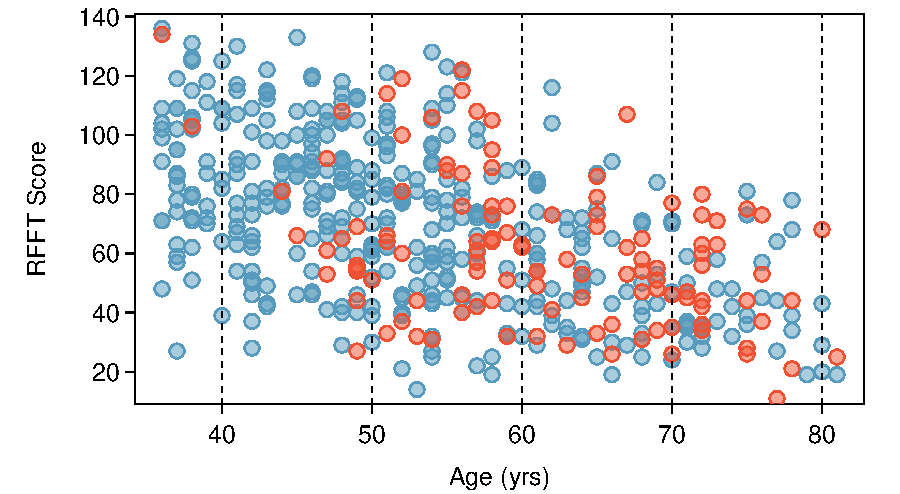
\includegraphics[width=0.85\textwidth]
	{ch_multiple_linear_regression_oi_biostat/figures/prevendAgeRFFTConfounderPlot/prevendAgeRFFTConfounderPlot}
	\caption{A scatterplot showing \var{age} vs. \var{RFFT} in \data{prevend.samp}. Statin users are represented with red points; participants not using statins are shown as blue points.}
	\label{prevendAgeRFFTConfounderPlot}
\end{figure}

Figure~\ref{prevendAgeRFFTConfounderPlot} visually demonstrates why age is a potential confounder for the association between statin use and cognitive function, where cognitive function is measured via the Ruff Figural Fluency Test (RFFT). Scores range from 0 (worst) to 175 (best). The blue points indicate individuals not using statins, while red points indicate statin users. First, it is clear that age and statin use are associated, with statin use becoming more common as age increases; the red points are more prevalent on the right side of the plot. Second, it is also clear that age is associated with lower RFFT scores; ignoring the colors, the point cloud drifts down and to the right. However, a close inspection of the plot suggests that for ages in relatively small ranges (e.g., ages 50-60), statin use may not be strongly associated with RFFT score\textemdash there are approximately as many red dots with low RFFT scores as with high RFFT scores. In other words, for subsets of participants with approximately similar ages, statin use may not be associated with RFFT. Multiple regression provides a way to estimate the association of statin use with RFFT after adjusting for age; essentially, it estimates the association of statin use and RFFT when age is 'held constant'.

\section{Simple versus multiple regression}
\label{simpleVsMultipleRegression}

A simple linear regression model can be fit for an initial examination of the association between statin use and RFFT score,
\[
E(\text{RFFT}) = \beta_0 + \beta_{\text{Statin}}(\text{Statin}).
\label{RFFTStatinModel}
\]

RFFT scores in \data{prevend.samp} are approximately normally distributed, ranging between approximately 10 and 140, with no obvious outliers (Figure~\ref{prevendRFFTHist}). The least squares regression line shown in Figure~\ref{prevendStatinRFFTDotPlot} has a negative slope, which suggests a possible negative association. 

\begin{figure}[ht]
	\centering
	\subfigure[]{
		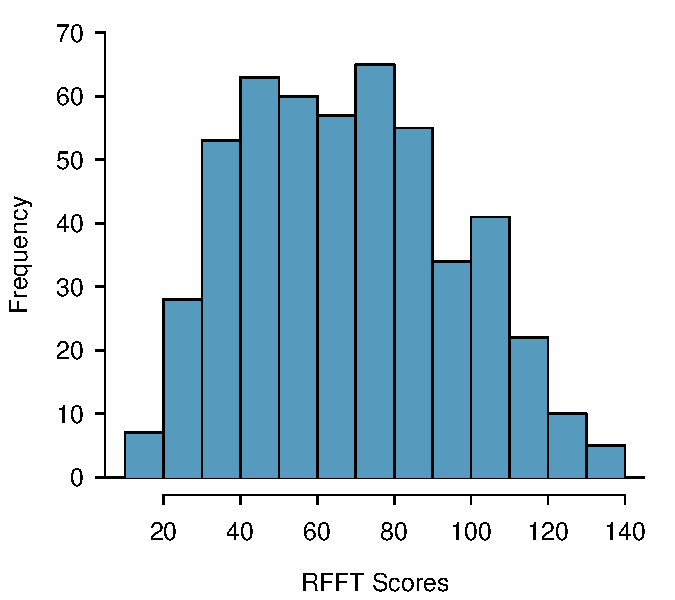
\includegraphics[width=0.40\textwidth]
		{ch_multiple_linear_regression_oi_biostat/figures/prevendStatinRFFTPlots/prevendRFFTHist}
		\label{prevendRFFTHist}
	}
	\subfigure[]{
		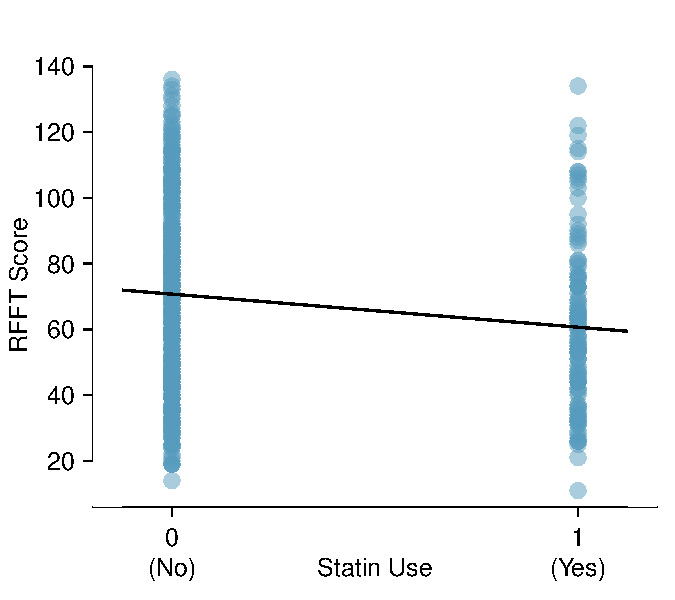
\includegraphics[width=0.40\textwidth]
		{ch_multiple_linear_regression_oi_biostat/figures/prevendStatinRFFTPlots/prevendStatinRFFTDotPlot}
		\label{prevendStatinRFFTDotPlot}
	}
	\caption{\subref{prevendRFFTHist} Histogram of RFFT scores. \subref{prevendStatinRFFTDotPlot} Scatterplot of RFFT score versus statin use in \data{prevend.samp}. The variable \var{Statin} is coded \resp{1} for statin users, and \resp{0} otherwise.}
	\label{prevendStatinRFFTPlot}
\end{figure}

Table~\ref{prevendRFFTStatinRegression} gives the parameter estimates of the least squares line, and indicates that the association between RFFT score and statin use is highly significant. On average, statin users score approximately 10 points lower on the RFFT. However, these results do not account for the effect of age. The clear linear trend in declining RFFT scores for older adults visible from Figure~\ref{prevendAgeRFFTConfounderPlot} is even more apparent in Figure~\ref{prevendStatinAgeBoxPlot}, where the median age of statin users is about 10 years higher than the median age of individuals not using statins. Even though the result from the initial model is statistically significant, it is potentially misleading since it ignores age.

% latex table generated in R 3.3.2 by xtable 1.8-2 package
% Fri Jan  5 10:49:51 2018
\begin{table}[ht]
\centering
\begin{tabular}{rrrrr}
  \hline
 & Estimate & Std. Error & t value & Pr($>$$|$t$|$) \\ 
  \hline
(Intercept) & 70.7143 & 1.3808 & 51.21 & 0.0000 \\ 
  Statin & -10.0534 & 2.8792 & -3.49 & 0.0005 \\ 
   \hline
\end{tabular}
\caption{\textsf{R} summary output for the simple regression model of RFFT versus statin use in \data{prevend.samp}.} 
\label{prevendRFFTStatinRegression}
\end{table}

 \begin{figure}[h]
 	\centering
 	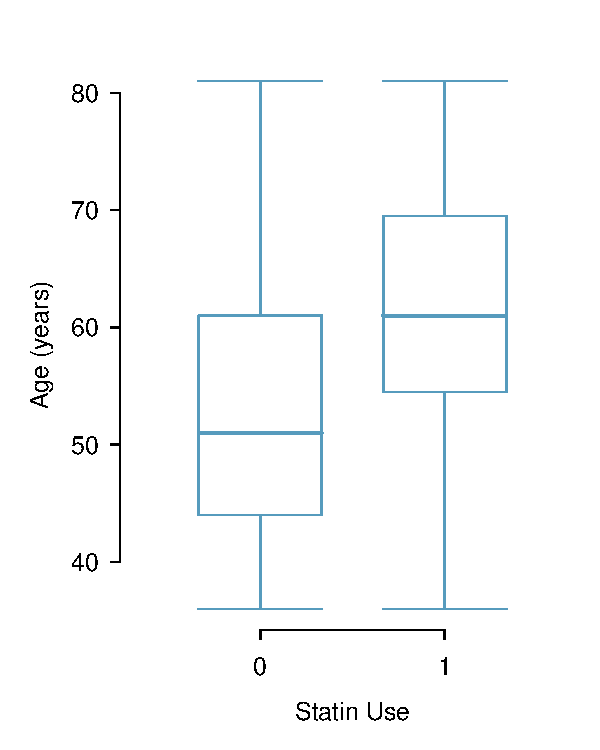
\includegraphics[width=0.45\textwidth]
 	{ch_multiple_linear_regression_oi_biostat/figures/prevendStatinAgeBoxPlot/prevendStatinAgeBoxPlot.pdf}
 	\caption{Boxplot of age by statin use in \data{prevend.samp}. The variable \var{Statin} is coded \resp{1} for statin users, and \resp{0} otherwise.}
 	\label{prevendStatinAgeBoxPlot}
 \end{figure}

%JV: removing the significance testing for RFFT vs age, since that is not the approach we are encouraging, generally

\begin{comment}

Even though the use of a statin drug explains only 2.4\% of the variability in the RFFT scores, the table does show that statin use is significantly associated with RFFT score. Statin users (those with value 1 in \var{statin}) score approximately 10 points lower on average in the RFFT test.  But the result may be confounded by age, as discussed earlier.   The boxplot in Figure~\ref{prevendStatinAgeBoxPlot} confirms that statin users tend to be older, and the scatterplot in Figure~\ref{prevendStatinAgeRFFTConfounderPlot} showed a clear linear trend in declining RFFT scores for older adults, regardless of statin use.  In fact, the regression output shown in Table~\ref{prevendRFFTAgeRegression} shows that age has a strongly significant association with RFFT score.
 
 \begin{figure}[h!]
 	\centering
 	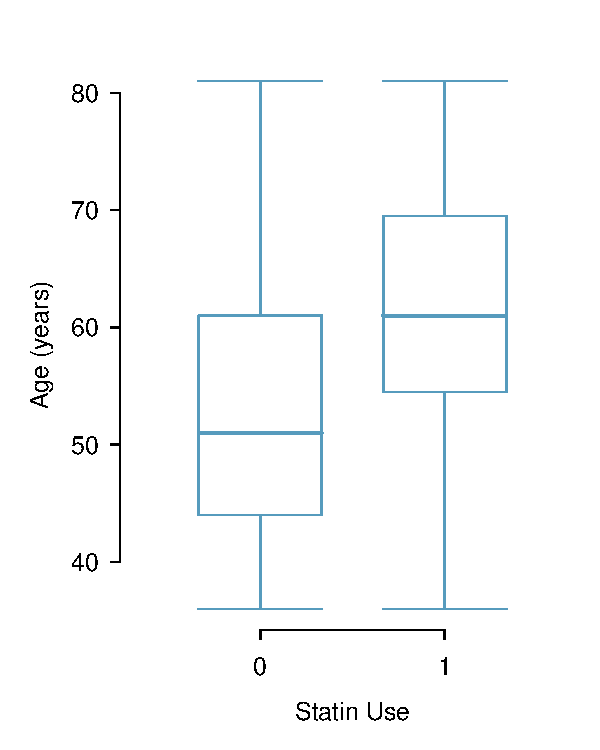
\includegraphics[width=0.4\textwidth]
	{ch_multiple_linear_regression_oi_biostat/figures/prevendStatinAgeBoxPlot/prevendStatinAgeBoxPlot.pdf}
 	\caption{Boxplot of age by statin use; 0 = participant not using statins, 1 = using statins. PREVEND data.}
	\label{prevendStatinAgeBoxPlot}
 \end{figure}
 
% latex table generated in R 3.3.2 by xtable 1.8-2 package
% Fri Jan  5 10:52:45 2018
\begin{table}[ht]
\centering
\begin{tabular}{rrrrr}
  \hline
 & Estimate & Std. Error & t value & Pr($>$$|$t$|$) \\ 
  \hline
(Intercept) & 137.5497 & 5.0161 & 27.42 & 0.0000 \\ 
  Age & -1.2614 & 0.0895 & -14.09 & 0.0000 \\ 
   \hline
\end{tabular}
\caption{R output from the regression of the 
       response variable RFFT with predictor Age} 
\label{prevendRFFTAgeRegression}
\end{table}
The model for multiple linear regression with two predictors is a straightforward extension of simple regression and can be used to adjust for confounders.  

\end{comment}

Multiple regression allows for a model that incorporates both statin use and age.
 \[
    E(\text{RFFT}) = \beta_0 + \beta_{\text{Statin}}(\text{Statin}) + \beta_{\text{Age}}(\text{Age}).
	\label{RFFTStatinAgeEquation}
 \]
In statistical terms, the association between \var{RFFT} and \var{Statin} is being estimated after adjusting for \var{Age}. This is an example of one of the more important applications of multiple regression: estimating an association between a response variable and primary predictor of interest while adjusting for possible confounders. In this setting, statin use is the primary predictor of interest.

The principles and assumptions behind the multiple regression model are introduced more formally in Section~\ref{generalMultipleRegression}, along with the method used to estimate the coefficients. Table~\ref{prevendRFFTStatinAgeRegression} shows the parameter estimates for the model from \textsf{R}. 
% latex table generated in R 3.3.2 by xtable 1.8-2 package
% Fri Jan  5 11:04:43 2018
\begin{table}[ht]
\centering
\begin{tabular}{rrrrr}
  \hline
 & Estimate & Std. Error & t value & Pr($>$$|$t$|$) \\ 
  \hline
(Intercept) & 137.8822 & 5.1221 & 26.92 & 0.0000 \\ 
  Statin & 0.8509 & 2.5957 & 0.33 & 0.7432 \\ 
  Age & -1.2710 & 0.0943 & -13.48 & 0.0000 \\ 
   \hline
\end{tabular}
\caption{\textsf{R} summary output for the multiple regression model of RFFT versus statin use and age in \data{prevend.samp}.} 
\label{prevendRFFTStatinAgeRegression}
\end{table}
 
\begin{example}{Using the parameter estimates in Table~\ref{prevendRFFTStatinAgeRegression}, write the prediction equation for the linear model. How does the predicted RFFT score for a 67-year-old not using statins compare to that of an individual of the same age who does use statins?}
	
The equation of the linear model is
\[\widehat{\text{RFFT}} = 137.8822 + 0.8509(\text{Statin}) - 1.2710(\text{Age}). \]	

The predicted RFFT score for a 67-year-old not using statins (\texttt{Statin = 0}) is
\[\widehat{\text{RFFT}} = 137.8822 + \textcolor{blue}{(0.8509)(0)} - (1.2710)(67) = 52.7252. \]

The predicted RFFT score for a 67-year-old using statins (\texttt{Statin = 1}) is
\[\widehat{\text{RFFT}} = 137.8822 + \textcolor{blue}{(0.8509)(1)} - (1.2710)(67) = 53.5761. \]


The two calculations differ only by the value of the coefficient $\beta_{\text{Statin}}$, 0.8509.\footnote{In most cases, predictions do not need to be calculated to so many significant digits, since the coefficients are only estimates. This example uses the additional precision to illustrate the role of the coefficients.} Thus, for two individuals who are the same age, the model predicts that RFFT score will be 0.8509 higher in the individual taking statins; statin use is associated with a small increase in RFFT score.
	
\end{example}

\begin{example}{Suppose two individuals are both taking statins; one individual is 50 years of age, while the other is 60 years of age. Compare their predicted RFFT scores.} 

From the model equation, the coefficient of age $\beta_{\text{Age}}$ is -1.2710; an increase in one unit of age (i.e., one year) is associated with a decrease in RFFT score of -1.2710, when statin use is the same. Thus, the individual who is 60 years of age is predicted to have an RFFT score that is about 13 points lower ($-1.2710(10) = -12.710$) than the individual who is 50 years of age. 

This can be confirmed numerically:

The predicted RFFT score for a 50-year-old using statins is
\[\widehat{\text{RFFT}} = 137.8822 + (0.8509)(1) - (1.2710)(50) = 75.1831. \]

The predicted RFFT score for a 60-year-old using statins is
\[\widehat{\text{RFFT}} = 137.8822 + (0.8509)(1) - (1.2710)(60) = 62.4731. \]

The scores differ by $62.4731 - 75.1831 = - 12.710.$
	
\end{example}

\begin{exercise} What does the intercept represent in this model? Does the intercept have interpretive value?\footnote{The intercept represents an individual with value \resp{0} for both \var{Statin} and \var{Age}; i.e., an individual not using statins with age of 0 years. It is not reasonable to predict RFFT score for a newborn, or to assess statin use; the intercept is meaningless and has no interpretive value.}
\end{exercise}

As in simple linear regression, $t$-statistics can be used to test hypotheses about the slope coefficients; for this model, the two null hypotheses are $H_0: \beta_{\text{Statin}} = 0$ and $H_0: \beta_{\text{Age}} = 0$. The $p$-values for the tests indicate that at significance level $\alpha = 0.05$, the association between RFFT score and statin use is not statistically significant, but the association between RFFT score and age is significant. The results of the analysis can be summarized as follows\textemdash

\begin{quotation}
	Although the use of statins appeared to be associated with lower RFFT scores when no adjustment was made for possible confounders, statin use is not significantly associated with RFFT score in a regression model that adjusts for age. The association of age with RFFT score is statistically significant; older participants tended to have lower scores.
\end{quotation}

The results shown in Table~\ref{prevendRFFTStatinAgeRegression} do not provide information about either the quality of the model fit or its potential value for making predictions. The next section describes the residual plots that can be used to check some of the model assumptions and the use of $R^2$ to estimate how much of the variability in the response variable is explained by the model.

There is an important aspect of these data that should not be overlooked. The data do not come from a study in which participants were followed as they aged; i.e., a longitudinal study. Instead, this study was a cross-sectional study, in which patient age, statin use, and RFFT score were recorded for all participants during a short time interval. While the results of the study support the conclusion that older patients tend to have lower RFFT scores, they cannot be used to conclude that scores decline with age in individuals; there was no measurement of RFFT changing over time as individual participants aged. Older patients come from an earlier birth cohort, and it is possible, for instance, that younger participants have more post-secondary school education or better health practices generally; such a cohort effect may have some explanatory effect on the observed association. The details of how a study is designed and how data are collected should always be taken into account when interpreting study results. 

\begin{comment}

\begin{itemize}
	
	\item The coefficients for \var{Statin} and \var{Age} can be used in a prediction.  The predicted RFFT score for a 67 year old using statins (\var{Statin} = 1) is 
	\[
	 \widehat{\text{RFFT}} = 137.822 + (0.8509)(1) - (1.2710)(67) = 53.5159.
	\]
The predicted RFFT for a 67 year old not using statins is
	\[
	 \widehat{\text{RFFT}} = 137.822 + (0.8509)(0) - (1.2710)(67) = 52.6650.
	\]
    The predicted RFFT score increases by 0.8509, the value of the \var{Statin} coefficient.  This is the most striking feature of the table -- in a model that includes \var{Age}, statin use seems to be associated with an increase in RFFT, rather than a decrease, as in the simple regression.

A simple calculation shows that this change in RFFT would have been the same for statin user vs non-user regardless of the value of \var{Age}, as long as the age is the same for the two participants. The coefficient for \var{Statin} is the change in predicted RFFT score for two individuals of the same age, but differing in whether they are taking statins.  In most cases, predictions are not calculated to so many significant digits, since the coefficients are only estimates.  This example uses the additional precision to illustrate the role of the coefficients.
	
	\item  Suppose neither of two participants was taking statins (\var{Statin} = 0), one 65 years old and the other 66.  The two predicted RFFT scores would be  55.207 and 53.936. The change in the predicted scores (-1.271) is the value of the coefficient for \var{Age}, because \var{Age} has changed by one year (one unit on the age scale).   A simple calculation shows that this predicted change would have been the same for two individuals 65 and 66 years old, both taking statins.  The coefficient for \var{Age} is the change in predicted RFFT score if age differs by one year and statin use is the same.
	
	\item Residuals in multiple regression are the differences between observed and predicted values for each case in the dataset, just as in simple regression.  In the sample of 500 cases used to estimate the regression model, there is a participant age 67, using statins, and whose RFFT score is 53.  The residual for that case would be $53 - 53.5150 = - 0.5159$.
	
 \item  The sign of the coefficients for the two predictors specifies the direction of change in the response RFFT when one of the predictors changes. Taking statins is associated with a small increase in RFFT score, while older age is associated with decreasing RFFT scores.
 
 \item  For each of the two coefficients, the $t$-statistic is the ratio of the estimated coefficient divided by its standard error.  Standard errors are more complicated to multiple regression than in simple regression, but they serve the same purpose.  They are an estimate of the standard deviation of the coefficient.  As in simple regression, the $t$-statistics can be used to test the two null hypotheses $H_0:\beta_{\text{Statin}} = 0$ or $H_0:\beta_{\text{Age}} = 0$ against two-sided alternatives.
  
  \item In a model with two predictors, the sampling distributions of the $t$-statistics for each of the parameters are $t$-distributions with $n - 2$ degrees of freedom, where $n$ is the number of cases used to estimate the regression. The last column in the table contains the two-sided $p$-values for these two hypothesis tests, just as in simple regression.  These $p$-values indicate that when using $\alpha = 0.05$ the association between statin use and RFFT score is not statistically significant, but the association between age and RFFT is significant.
  
  \item  The result of the analysis can be summarized with the statement, ``Although the use of statins appeared to be associated with lower RFFT scores when no adjustment has been made for possible confounders, statins are not significantly associated with RFFT score in a regression model that adjusts for age.  The association of age with RFFT is statistically significant; older participants had lower scores.''
  
  \item Just as in simple linear regression, the coefficient for the intercept must be interpreted with care.  In this model, the intercept gives the predicted RFFT for someone not using statins and of age 0, and is clearly meaningless.
  
  \item There is an important aspect of these data that should not be overlooked.  The data do not come from a study in which participants were followed as they aged, allowing for the measurement of changing RFFT in a participant over time. Such a study is called a longitudinal study.  This study was a cross-sectional study -- patient age, statin use and RFFT were recorded for all participants during a short time interval.  The results of the study support the conclusion that older patients tend to have lower RFFT scores, but cannot be used to conclude that scores decline with age in individuals.  Older patients come from an earlier birth cohort, and it is possible, for instance, that younger participants have more post-secondary school education or better health practices generally.  In other words, there may be a cohort effect.  This is an important point to be aware of, and is not at all evident in the Table~\ref{prevendRFFTStatinAgeRegression}
  
 \end{itemize}
 
 
The results of the analysis shown in Table~\ref{prevendRFFTStatinAgeRegression} provide an initial look at the association between RFFT score, statin use and age. There is, however, no information about either the quality of the fit or its potential value for predictions. The next section describes the residual plots that can be used to check some of the model assumptions and the use of $R^2$ to estimate how much of the variability in the response variable is explained by the model.

\end{comment}

\section{Evaluating the fit of a multiple regression model}

\subsection{Using residuals to check model assumptions}

The assumptions behind multiple regression are essentially the same as the four assumptions listed in Section~\ref{examiningScatterplots} for simple linear regression. The assumption of linearity is extended to multiple regression by assuming that when only one predictor variable changes, it is linearly related to the change in the response variable.  Assumption 2 becomes the slightly more general assumption that the residuals have approximately constant variance. Assumptions 3 and 4 do not change: the observations on each case are independent, and the residuals are approximately normally distributed.

Since it is not possible to make a scatterplot of a response variable against several simultaneous predictors, residual plots become even more essential as tools for checking modeling assumptions. 

To assess the linearity assumption, examine plots of residuals against each of the predictors. These plots might show an nonlinear trend that could be corrected with a transformation. The scatterplot of residuals versus age in Figure~\ref{prevendStatinAgeResidPlot} shows no apparent nonlinear trends. It is not necessary to assess linearity against a categorical predictor, since a line drawn through two points (i.e., the means of the two groups) is necessarily linear.

\begin{figure}[h!]
	\centering
	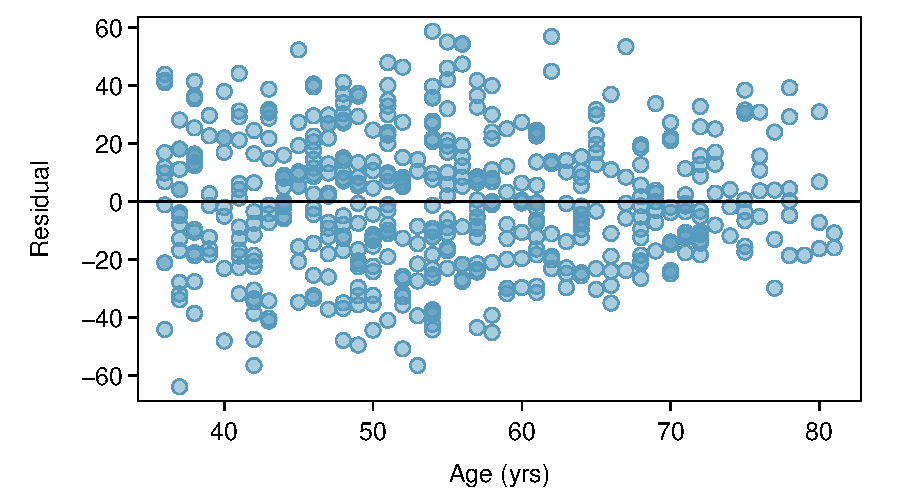
\includegraphics[width=0.8\textwidth]
	{ch_multiple_linear_regression_oi_biostat/figures/prevendStatinAgeResidPlot/prevendStatinAgeResidPlot.pdf}
	\caption{Age vs residuals in the model for RFFT vs statins and age in the PREVEND data.  The horizontal line is the least squares line for age vs the residuals.}
	\label{prevendStatinAgeResidPlot}
\end{figure}

Since each case has one predicted value and one residual, regardless of the number of predictors, residuals can still be plotted against predicted values to assess the constant variance assumption. The patterns that might indicate lack of fit are the same as in Figure~\ref{sampleLinesAndResPlots} from Chapter~\ref{linRegrForTwoVar}. The scatterplot in the left panel of Figure~\ref{prevendStatinAgeResidNormPlot} shows that the variance of the residuals is slightly smaller for low predicted values of RFFT, but is otherwise approximately constant.

Just as in simple regression, normal probability plots can be used to check the normality assumption of the residuals. The normal probability plot in the right panel of Figure~\ref{prevendStatinAgeResidNormPlot} shows that the residuals from the model are reasonably normally distributed, with only slight departures from normality in the tails.

\begin{figure}[h!]
	\centering
	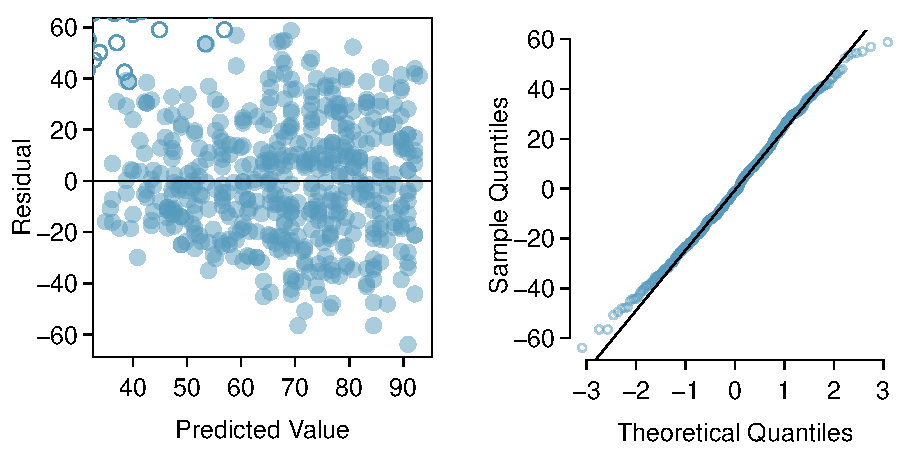
\includegraphics[width=0.8\textwidth]
	{ch_multiple_linear_regression_oi_biostat/figures/prevendStatinAgeResidNormPlot/prevendStatinAgeResidNormPlot.pdf}
	\caption{Residual plots from the linear model for RFFT versus statin use and age in \data{prevend.samp}.}
	\label{prevendStatinAgeResidNormPlot}
\end{figure}

\begin{example}{Section~\ref{exploratoryDataAnalysis} featured a case study examining the evidence for ethnic discrimination in the amount of financial support offered by the State of California to individuals with developmental disabilities. Although an initial look at the data suggested an association between \var{expenditures} and \var{ethnicity}, further analysis suggested that age is a confounding variable for the relationship.

Suppose a multiple regression model is fit to these data to model the association between \var{expenditures}, \var{age}, and \var{ethnicity}; the dataset \data{dds.discr} has been subsetted to only include data from Hispanics and White non-Hispanics, the two groups studied in the Chapter~\ref{introductionToData}	analysis. Two residual plots from the model fit for 
\[E(\text{expenditures}) = \beta_0 +  \beta_{\text{ethnicity}}(\text{ethnicity}) + \beta_{\text{age}}(\text{age}) \]
are shown in Figure~\ref{ddsAgeEthnicityResidNormPlot}. From these plots, assess whether the model assumptions are met. 

\begin{figure}[h!]
	\centering
	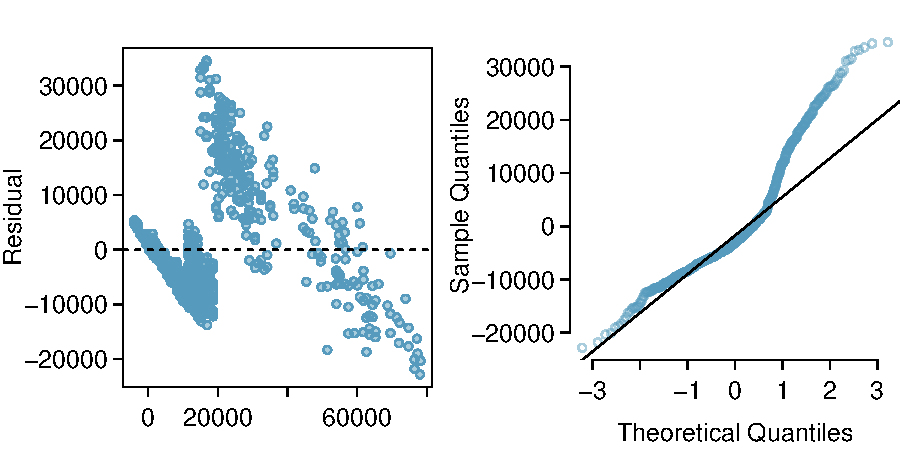
\includegraphics[width=0.85\textwidth]
	{ch_multiple_linear_regression_oi_biostat/figures/ddsAgeEthnicityResidNormPlot/ddsAgeEthnicityResidNormPlot.pdf}
	\caption{Residual versus fitted values plot and residual normal probability plot from the linear model for expenditures versus ethnicity and age for a subset of \data{dds.discr}.}
	\label{ddsAgeEthnicityResidNormPlot}
\end{figure}		
		
%JV: 12Jan2018, cannot figure out how to adjust margins so that x-labels show without y-labels running into y tick-labels...
		
}

The model assumptions are clearly violated. The residual versus fitted plot	shows obvious patterns; the residuals do not scatter randomly about the $y = 0$ line. Additionally, the variance of the residuals is not constant around the $y = 0$ line. As shown in the normal probability plot, the residuals show marked departures from normality, particularly in the upper tail; although this skewing may be partially resolved with a log transformation, the patterns in the residual versus fitted plot are more problematic.

Recall that a residual is the difference between an observed value and expected value; for an observation $i$, the residual equals $y_i - \hat{y}_i$. Positive residuals occur when a model's predictions are larger than the observed value, and vice versa for negative residuals. In the residual versus fitted plot, it can be seen that in the middle range of predicted values, the model consistently underpredicts expenditures; on the upper and lower ends, the model overpredicts. This is a particularly serious issue with the model fit. 

A linear regression model is not appropriate for these data.	
	
\end{example}


\subsection{Using $R^2$ and adjusted $R^2$ with multiple regression}
\index{adjusted r squared@adjusted $R^2$ ($R_{adj}^2$)|(}

Section~\ref{RSquaredLinearRegression} provided two definitions of the $R^2$ statistic\textemdash it is the square of the correlation coefficient $r$ between a response and the single predictor in simple linear regression, and equivalently, it is the proportion of the variation in the response variable explained by the model.  In statistical terms, the second definition can be written as 
\[
   R^2 = \frac{\text{Var}(y_i) - \text{Var}(e_i)}
   {\text{Var}(y_i)} = 1 - \frac{\text{Var}(e_i)}{\text{Var}(y_i)},
   \label{RSquareDefinition}\]
where $y_i$ and $e_i$ denote the response and residual values for the
$i^{\text{th}}$ case.

The first definition cannot be used in multiple regression, since there is a correlation coefficient between each predictor and the response variable. However, since there is a single set of residuals, the second definition remains applicable. 

Although $R^2$ can be calculated directly from the equation, it is rarely calculated by hand since computing software includes $R^2$ as a standard part of the summary output for a regression model.\footnote{In \textsf{R} and other softwares, $R^2$ is typically labeled 'multiple R-squared'.} The model with In the model with response \var{RFFT} and predictors \var{Statin} and \var{Age}, $R^2 = 0.2852$.  The model explains almost 29\% of the variability in RFFT scores, a considerable improvement over the model with \var{Statin} alone ($R^2 = 0.0239$).

Advanced courses in regression show that adding a variable to a regression model always increases the value of $R^2$. Sometimes that increase is large and clearly important, such as when \var{Age} is added to the model for RFFT scores. In other cases, the increase is small, and may not be worth the added complexity of including another variable. The \term{adjusted R-squared} is often used to balance predictive ability with complexity in a multiple regression model. Like $R^2$, the adjusted $R^2$ is routinely provided in software output. 

\begin{termBox}{\tBoxTitle{Adjusted $\mathbf{R^2}$ as a tool for model assessment}
The \termsub{adjusted $\mathbf{R^2}$}{adjusted r squared@adjusted $R^2$ ($R_{adj}^2$)} is computed as
\begin{align*}
R_{adj}^{2} = 1-\frac{\text{Var}(e_i) / (n-p-1)}{\text{Var}(y_i) / (n-1)}
	= 1-\frac{\text{Var}(e_i)}{\text{Var}(y_i)} \times
    \frac{n-1}{n-p-1},
\end{align*}
where $n$ is the number of cases used to fit the model and $p$ is the number of predictor variables in the model.}
\end{termBox}

Since $p = 1$ in simple linear regression, the $R^2$ and adjusted $R^2$ have the same value when there is only a single predictor. 

Essentially, the adjusted $R^2$ imposes a penalty for including additional predictors that do not contribute much towards explaining the observed variation in the response variable. The value of the adjusted $R^2$ in the model with both \var{Statin} and \var{Age} is 0.2823\textemdash the additional predictor \var{Age} adds only moderate complexity while increasing the strength of model considerably, relative to the model with only \var{Statin}.

While the adjusted $R^2$ is useful as a statistic for comparing models, it does not have an inherent interpretation like $R^2$. Students often confuse the interpretation of $R^2$ and adjusted $R^2$; while the two are similar, adjusted $R^2$ is \emph{not} the proportion of variation in the response variable explained by the model. The use of adjusted $R^2$ for model selection will be discussed in Section~\ref{modelSelectionPrediction}.

%DH: \textit{guided practice to calculate adjusted R-squared by hand could be inserted here}
%JV: perhaps not that valuable without an explanation of why (n-1)/(n-p-1) as a penalty

 
 \section{The general multiple linear regression model}
 \label{generalMultipleRegression}
 
Sections~\ref{introductionMultipleLinearRegression} and \ref{simpleVsMultipleRegression} introduced multiple regression with two predictors as a technique to estimate an association of primary interest in the presence of confounding.  Multiple regression has many more applications\textemdash it can be used to build a model for prediction responses, for learning which subset of variables in a set of potential predictors are associated with the response, and as a unified approach to ANOVA.

This section provides a compact summary of the multiple regression model and contains more mathematical detail than most other sections; the next section, Section~\ref{categoricalMoreThanTwoLevels}, discusses categorical predictors with more than two levels. The ideas outlined in this section and the next are illustrated with an extended analysis of the PREVEND data in Section~\ref{reanalyzingStatinDataSet}. 
 
\subsection{Model parameters and least squares estimation}
 
For multiple regression, the data consist of a response variable $Y$ and $p$ potential predictors or explanatory variables $X_1, X_2,\ldots, X_p$.   Instead of the simple regression model 
 $${Y} = \beta_{0} + \beta_{1}X + {\varepsilon},$$
 multiple regression has the form
 $${Y} = \beta_{0} +
     \beta_{1}X_{1} + \beta_{2}X_{2} + \beta_{3}X_{3} + \dots +
     \beta_{p}X_{p} + \varepsilon,$$
or equivalently
 $$E(Y) = \beta_{0} + 
     \beta_{1}X_{1} + \beta_{2}X_{2} + \beta_{3}X_{3} + \dots +
     \beta_{p}X_{p},
	 \label{multipleRegressionModel}
	 $$ 
since the normally distributed error term $\varepsilon$ is assumed to have mean 0. Each predictor $x_i$ has an associated coefficient $\beta_i$.  In simple regression, the slope coefficient $\beta$ captures the change in the response variable $Y$ associated with a one unit change in the predictor $X$.  In multiple regression, the coefficient $\beta_j$ of a predictor $X_j$ denotes the change in the response variable $Y$ associated with a one unit change in $X_j$ when none of the other predictors change; i.e., each $\beta$ coefficient in multiple regression plays the role of a slope, as long as the other predictors are not changing.

Multiple regression can be thought of as the model for the mean of the response $Y$ in a population where the mean depends on the values of the predictors, rather than being constant. For example, consider a setting with two binary predictors such as statin use and sex; the predictors partition the population into four subgroups, and the four predicted values from the model are estimates of the mean in each of the four groups.

\begin{exercise}
Table~\ref{prevendRFFTStatinGenderRegression} shows an estimated regression model for \var{RFFT} with predictors \var{Statin} and \var{Gender}, where \var{Gender} is coded 0 for males and 1 for females.\footnote{Until recently, it was common practice to use \var{gender} to denote biological sex. Gender is different than biological sex, but this text uses the original names in published datasets.}  Based on the model, what are the estimated mean RFFT scores for the four groups defined by these two categorical predictors?\footnote{The prediction equation for the model is $\widehat{\text{RFFT}} = 70.41 - 9.97(\text{Statin}) + 0.61(\text{Gender})$. Both \texttt{Statin} and \texttt{Gender} can take on values of either \resp{0} or \resp{1}; the four possible subgroups are statin non-user / male (\texttt{0}, \texttt{0}), statin non-user / female (\texttt{0}, \texttt{1}), statin user / male (\texttt{1}, \texttt{0}), statin user / female (\texttt{1}, \texttt{1}). Predicted RFFT scores for these groups are 70.41, 71.02, 60.44, and 61.05, respectively.} 
% latex table generated in R 3.3.2 by xtable 1.8-2 package
% Fri Jan  5 11:21:50 2018
\begin{table}[ht]
\centering
\begin{tabular}{rrrrr}
  \hline
 & Estimate & Std. Error & t value & Pr($>$$|$t$|$) \\ 
  \hline
(Intercept) & 70.4068 & 1.8477 & 38.11 & 0.0000 \\ 
  Statin & -9.9700 & 2.9011 & -3.44 & 0.0006 \\ 
  Gender & 0.6133 & 2.4461 & 0.25 & 0.8021 \\ 
   \hline
\end{tabular}
\caption{\textsf{R} summary output for the multiple regression model of RFFT versus statin use and sex in \data{prevend.samp}.}
\label{prevendRFFTStatinGenderRegression}
\end{table}
\end{exercise}

Datasets for multiple regression have $n$ cases, usually indexed algebraically by $i$, where $i$ takes on values from 1 to $n$, where 1 denotes the first case in the dataset and $n$ denotes the last case.  The dataset \data{prevend.samp} contains $n = 500$ observations.  Algebraic representations of the data must indicate both the case number and the predictor in the set of $p$ predictors. For case $i$ in the dataset, the variable $X_{ij}$ denotes predictor $X_j$; the response for case $i$ is simply $Y_i$, since there can only be one response variable. The dataset \data{prevend.samp} has many possible predictors, some of which are examined later in this chapter.  The analysis in Section~\ref{simpleVsMultipleRegression} used $p=2$ predictors, \var{Statin} and \var{Age}.

Just as in Chapter~\ref{probability}, upper case letters are used when thinking of data as a set of random observations subject to sampling from a population, and lower case letters are used for observed values. In a dataset, it is common for each row to contain the information on a single case; the observations in row $i$ of a dataset with $p$ predictors can be written as $(y_i, x_{i1}, x_{i2}, \ldots, x_{ip})$.

For any given set of estimates $b_1, b_2,\ldots,b_p$ and predictors $x_{i1},x_{i2},\ldots,x_{ip}$, predicted values of the response can be calculated using
\[
   \hat{y}_i = b_0 + b_1 x_{i1} + b_2 x_{i2} +\cdots b_p x_{ip},
\]

where $b_0, b_1, \dots, b_p$ are estimates of the coefficients $\beta_0, \beta_1, \dots, \beta_p$ obtained using the principle of least squares estimation. As in simple regression, each prediction has an associated residual, which is the difference between the observed value $y_i$ and the predicted value $\hat{y_i}$, or $e_i = y_i - \hat{y}_i$. The least squares estimate of the model is the set of estimated coefficients $b_0, b_1, \ldots b_p$ that minimizes $e_1^2 + e_2^2 + \cdots e_n^2$. Explicit formulas for the estimates involve advanced matrix theory, but are rarely used in practice.  Instead, estimates are calculated using software such as as \textsf{R}, Stata, or Minitab.

\subsection{Hypothesis tests and confidence intervals}

\subsubsection{Using $t$-tests for individual coefficients}

The test of the null hypothesis $H_0: \beta_j = 0$ is a test of whether the predictor $X_j$ is associated with the response variable. When a coefficient of a predictor equals 0, the predicted value of the response does not change when the predictor changes; i.e., a value of 0 indicates there is no association between the predictor and response. Due to the inherent variability in observed data, an estimated coefficient $b_j$ will almost never be 0 even when the model coefficient $\beta_j$ is. Hypothesis testing can be used to assess whether the estimated coefficient is significantly different from 0 by examining the ratio of the estimated coefficient to its standard error.


When the assumptions of a multiple regression hold, at least approximately, this ratio has a $t$-distribution with $n - (p + 1) =n - p - 1$ degrees of freedom when the model coefficient is 0. The formula for the degrees of freedom follows a general rule that appears throughout statistics\textemdash the degrees of freedom for an estimated model is the number of cases in the dataset minus the number of estimated parameters.  There are $p + 1$ parameters in the multiple regression model, one for each of the $p$ predictors and one for the intercept.

\begin{termBox}{\tBoxTitle{Sampling distributions of estimated coefficients}
Suppose 
\[
\hat{y} = b_0 + b_1 x_{i} + b_2 x_{i} +\cdots b_p x_{i}
\]
is an estimated multiple regression model from a dataset with $n$ observations on the response and predictor variables, and let $b_k$ be one of the estimated coefficients.  Under the hypothesis $H_0: \beta_k = 0$, the standardized statistic
\[
      \frac{b_k}{\textrm{s.e.}(b_k)}
\]
has a $t$-distribution with $n - p - 1$ degrees of freedom.}
\end{termBox}

This sampling distribution can be used to conduct hypothesis tests and construct confidence intervals.

\begin{termBox}{\tBoxTitle{Testing a hypothesis about a regression coefficient}
A test of the two-sided hypothesis
\[
  H_0: \beta_k = 0 \text{ vs. } H_A: \beta_k \ne 0
\]
is rejected with significance level $\alpha$ when 
\[
     \frac{|b_k|}{\textrm{s.e.}(b_k)} > t_{\text{df}}^\star,
\]
where $t_{\text{df}}^\star$ is the point on a $t$-distribution with $n - p - 1$ degrees of freedom and area $(1 - \alpha/2)$ in the left tail.}
\end{termBox}

For one-sided tests, $t_{\text{df}}^\star$ is the point on a $t$-distribution with $n - p - 1$ degrees of freedom and area $(1 - \alpha)$ in the left tail. A one-sided test of $H_0$ against $H_A: \beta_k > 0$ rejects when the standardized coefficient is greater than  $ t_{\text{df}}^\star$; a one-sided test of $H_0$ against $H_A: \beta_k < 0$  rejects when the standardized coefficient is less than $-t_{\text{df}}^\star$. 

\begin{termBox}{\tBoxTitle{Confidence intervals for regression coefficient}
A two-sided $100(1 - \alpha)$\% confidence interval for the model coefficient $\beta_k$ is 
\[
     b_k \pm {\textrm{s.e.}(b_k)} \times t_{\text{df}}^\star.
\]}
\end{termBox}


\subsubsection{The $F$-statistic for an overall test of the model}

When all the model coefficients are 0, the predictors in the model, considered as a group, are not associated with the response; i.e., the response variable is not associated with any linear combination of the predictors. The $F$-statistic is used to test this null hypothesis of no association, using the following idea.  

The variability of the predicted values about the overall mean response can be estimated by
\[
   \text{MSM} =  \frac{\sum_i(\hat{y}_i - \overline{y})^2}{p}.
\]
In this expression, $p$ is the number of predictors and is the degrees of freedom of the numerator sum of squares (derivation not given here).  The term \term{MSM} is called the model sum of squares because it reflects the variability of the values predicted by the model ($\hat{y_i}$) about the mean ($\overline{y}$) response.\footnote{It turns out that $\overline{y}$ is also the mean of the predicted values.} In an extreme case, MSM will have value 0 when all the predicted values coincide with the overall mean; in this scenario, a model would be unnecessary for making predictions, since the average of all observations could be used to make a prediction.

The variability in the residuals can be measured by 
\[
  \text{MSE} = \frac{\sum_i(y_i - \hat{y}_i)^2}{n - p - 1}.
\]
\term{MSE} is called the mean square of the errors since residuals are
the observed `errors', the differences between predicted and observed
values.

When MSM is small compared to MSE, the model has captured little of the variability in the data, and the model is of little or no value.  The $F$-statistic is given by
\[
  F = \frac{\text{MSM}}{\text{MSE}}.
\]

The formula is not used for calculation, since the numerical value of the $F$-statistic is a routine part of the output of regression software.

\begin{termBox}{\tBoxTitle{The $F$-statistic in regression}
The $F$-statistic in regression is used to test the null hypothesis 

\[
  H_0:\, \beta_1 = \beta_2 = \cdots \beta_p = 0
\]
against the alternative that at least one of the coefficients is not 0.

Under the null hypothesis, the sampling distribution of the $F$-statistic is an $F$-distribution with parameters $(p, n - p - 1)$, and the null hypothesis is rejected if the value of the $F$-statistic is in the right tail of the distribution of the sampling distribution with area $\alpha$, where $\alpha$ is the significance level of the test.}
\end{termBox}

The $F$-test is inherently one-sided\textemdash deviations from the null hypothesis of any form will push the statistic to the right tail of the $F$-distribution.  The $p$-value from the right tail of the $F$-distribution should never be doubled.  Students also sometimes make the mistake of assuming that if the null hypothesis of the $F$-test is rejected, all coefficients must be non-zero, instead of at least one. A significant $p$-value for the $F$-statistic suggests that the predictor variables in the model, when considered as a group, are associated with the response variable.

In practice, it is rare for the $F$-test not to reject the null hypothesis, since most regression models are used in settings where a scientist has some prior evidence that at least some of the predictors are useful.

\begin{comment}

Since the two parameters are associated with the numerator and denominator of the $F$-statistic, the two degrees of freedom for an $F$-test are often referred to as the numerator and denominator degrees of freedom.

\end{comment}

\section{Categorical predictors with more than two levels}
\label{categoricalMoreThanTwoLevels}

In the initial model fit with the PREVEND data, the variable \var{Statin} is coded \resp{0} if the participant was not using statins, and coded \resp{1} if the participant was a statin user. The category coded \resp{0} is referred to as the reference category; in this model, statin non-users (\var{Statin = 0}) are the reference category. The estimated coefficient $\beta_{\text{Statin}}$ is the change in the average response between the reference category and the category \var{Statin = 1}.

Since the variable \var{Statin} is categorical, the numerical codes \resp{0} and \resp{1} are simply labels for statin non-users and users. The labels can be specified more explicitly in software. For example, in \textsf{R}, categorical variables can be coded as factors; the levels of the variable are displayed as text (such as "NonUser" or "User"), while the data remain stored as integers. The \textsf{R} output with the variable \var{Statin.factor} is shown in Table~\ref{prevendRFFTStatinFactorRegression}, where \resp{0} corresponds to the label "NonUser" and \resp{1} corresponds to "User". The predictor variable is now labeled \var{Statin.factorUser}; the estimate -10.05 is the change in mean RFFT from the "NonUser" (reference) category to the "User" category. Note how the reference category is not explicitly labeled; instead, it is contained within the intercept. 

% latex table generated in R 3.3.2 by xtable 1.8-2 package
% Fri Jan  5 11:27:38 2018
\begin{table}[ht]
	\centering
	\begin{tabular}{rrrrr}
		\hline
		& Estimate & Std. Error & t value & Pr($>$$|$t$|$) \\ 
		\hline
		(Intercept) & 70.7143 & 1.3808 & 51.21 & 0.0000 \\ 
		 Statin.factorUser & -10.0534 & 2.8792 & -3.49 & 0.0005 \\ 
		\hline
	\end{tabular}
	\caption{\textsf{R} summary output for the simple regression model of RFFT versus statin use in \data{prevend.samp}, with \var{Statin} converted to a factor called \var{Statin.factor} that has levels \texttt{NonUser} and \texttt{User}.} 
	\label{prevendRFFTStatinFactorRegression}
\end{table}

For a categorical variable with two levels, estimates from the regression model remain the same regardless of whether the categorical predictor is treated as numerical or not. A "one unit change" in the numerical sense corresponds exactly to the switch between the two categories. However, this is not true for categorical variables with more than two levels. 

This idea will be explored with one of the categorical variables in the PREVEND data, \var{Education}, which indicates the highest level of education that an individual completed in the Dutch educational system: primary school, lower secondary school, higher secondary education, or university education. In the PREVEND dataset, educational level is coded as either \resp{0}, \resp{1}, \resp{2}, or \resp{3}, where \resp{0} denotes at most a primary school education, \resp{1} a lower secondary school education, \resp{2} a higher secondary education, and \resp{3} a university education.

Just as in the two-category setting, one of the categories is set as the reference category. The remaining categories each have an estimated coefficient, which corresponds to the estimated change in response relative to the reference category. 

\begin{example}{Is RFFT score associated with educational level? Interpret the coefficients from the following model. Table~\ref{prevendRFFTEducationRegression} provides the \textsf{R} output for the regression model of RFFT versus educational level in \data{prevend.samp}. The variable \var{Education} has been converted to \var{Education.factor}, which has levels \texttt{Primary}, \texttt{LowerSecond}, \texttt{HigherSecond}, and \texttt{Univ}.
		
% latex table generated in R 3.3.2 by xtable 1.8-2 package
% Fri Jan  5 11:32:59 2018
\begin{table}[ht]
	\centering
	\begin{tabular}{rrrrr}
		\hline
		& Estimate & Std. Error & t value & Pr($>$$|$t$|$) \\ 
		\hline
		(Intercept) & 40.9412 & 3.2027 & 12.78 & 0.0000 \\ 
		Education.factorLowerSecond & 14.7786 & 3.6864 & 4.01 & 0.0001 \\ 
		Education.factorHigherSecond & 32.1335 & 3.7631 & 8.54 & 0.0000 \\ 
		Education.factorUniv & 44.9639 & 3.6835 & 12.21 & 0.0000 \\ 
		\hline
	\end{tabular}
	\caption{\textsf{R} summary output for the regression model of RFFT versus educational level in \data{prevend.samp}, with \var{Education} converted to a factor called \var{Education.factor} that has levels \texttt{Primary}, \texttt{LowerSecond}, \texttt{HigherSecond}, and \texttt{Univ}.}
		\label{prevendRFFTEducationRegression}
\end{table}		
		
}

It is clearest to start with writing the model equation:
\[\widehat{\text{RFFT}} =  40.94 + 14.78(\text{EduLowerSecond}) + 32.13(\text{EduHigherSecond}) + 44.96(\text{EduUniv})\]

Each of the predictor levels can be thought of as binary variables that can take on either \resp{0} or \resp{1}, where only one level at most can be a \resp{1} and the rest must be \resp{0}, with \resp{1} corresponding to the category of interest. For example, the predicted mean RFFT score for individuals in the Lower Secondary group is given by
\[\widehat{\text{RFFT}} =  40.94 + 14.78(1) + 32.13(0) + 44.96(0) = 55.72. \]
The value of the \texttt{LowerSecond} coefficient, 14.78, is the change in predicted mean RFFT score from the reference category \texttt{Primary} to the \texttt{LowerSecond} category. 

Participants with a higher secondary education scored approximately 32.1 points higher on the RFFT than individuals with only a primary school education, and have estimated mean RFFT score $40.94 + 32.13 = 73.07.$ Those with a university education have estimated mean RFFT score $40.94 + 44.96 = 85.90$.  

The intercept value, 40.94, corresponds to the estimated mean RFFT score for individuals who at most completed primary school. From the regression equation, 
\[\widehat{\text{RFFT}} =  40.94 + 14.78(0) + 32.13(0) + 44.96(0) = 40.94. \]

The $p$-values indicate that the change in mean score between participants with only a primary school education and any of the other categories is statistically significant.

\end{example}

\begin{example}{Suppose that the model for predicting RFFT score from educational level is fitted with \var{Education}, using the original numerical coding with \resp{0}, \resp{1}, \resp{2}, and \resp{3}; the \textsf{R} output is shown in Table~\ref{prevendRFFTEducationNumRegression}. What does this model imply about the change in mean RFFT between groups? Explain why this model is flawed.
		
\begin{table}[ht]
	\centering
	\begin{tabular}{rrrrr}
		\hline
		& Estimate & Std. Error & t value & Pr($>$$|$t$|$) \\ 
		\hline
		(Intercept) & 41.148 & 2.104 & 19.55 & 0.0000 \\ 
		Education & 15.158 & 1.023 & 14.81 & 0.0000 \\ 
		\hline
	\end{tabular}
	\caption{\textsf{R} summary output for the simple regression model of RFFT versus educational level in \data{prevend.samp}, where \var{Education} is treated as a numerical variable. Note that it would be incorrect to fit this model; Table~\ref{prevendRFFTEducationRegression} shows the results from the correct approach.} 
	\label{prevendRFFTEducationNumRegression}
\end{table}
		
}
	
According to this model, the change in mean RFFT between groups increases by 15.158 for any one unit change in \var{Education}. For example, the change in means between the groups coded \resp{0} and \resp{1} is necessarily equal to the change in means between the groups coded \resp{2} and \resp{3}, since the predictor changes by 1 in both cases. 

It is unreasonable to assume that the change in mean RFFT score when comparing the primary school group to the lower secondary group will be equal to the difference in means between the higher secondary group and university group. The numerical codes assigned to the groups are simply short-hand labels, and are assigned arbitrarily. As a consequence, this model would not provide consistent results if the numerical codes were altered; for example, if the primary school group and lower secondary group were relabeled such that the predictor changes by 2, the estimated difference in mean RFFT would change. 

\end{example}

Categorical variables can be included in multiple regression models with other predictors, as is shown in the next section. Section~\ref{ANOVAandRegression} discusses the connection between ANOVA and regression models with only one categorical predictor.


\begin{comment}

In the model~\ref{RFFTStatinModel}, the variable \var{Statin} is a categorial predictor with two values, coded 0 if the participant was not taking a statin, and 1 if he or she was using the medication.  Without adjusting for age, the estimated coefficient (-10.05) suggests that taking a statin may be associated with a 10 point drop in RFFT score.  In a model such as this, the category \var{Statin = 0} is called the reference category, and the estimated coefficient is the change in the average response between the category \var{Statin = 1} and the reference category.

Software such as \textsf{R} includes the option of declaring categorical variables as factors, with values (called levels) that serve as labels for categories instead of as numerical values.  Here is the output from \textsf{R} of a regression of RFFT score with the predictor \var{Statin} declared as a factor:
% latex table generated in R 3.3.2 by xtable 1.8-2 package
% Fri Jan  5 11:27:38 2018
\begin{table}[ht]
\centering
\begin{tabular}{rrrrr}
  \hline
 & Estimate & Std. Error & t value & Pr($>$$|$t$|$) \\ 
  \hline
(Intercept) & 70.7143 & 1.3808 & 51.21 & 0.0000 \\ 
  as.factor(Statin)1 & -10.0534 & 2.8792 & -3.49 & 0.0005 \\ 
   \hline
\end{tabular}
\caption{Parameter estimates for 
       the least squares regression of RFFT vs. 
       statin use,  with \var{Statin} converted to a 
       factor variable.  PREVEND Data.} 
\end{table}

The predictor is now labeled \texttt{as.factor(Statin)1}, denoting that the value 0 is the reference category, since the estimate -10.05 is the change in mean RFFT when the category for \var{Statin} changes from 0 to 1.  The regression estimate is the same as in the model where \var{Statin} was treated as a numerical value, because in that instance a 1 unit change in \var{Statin} was a change in mean RFFT between not taking a statin to taking one.  

The same idea is used when estimating the association of a response with a categorical variable that has more than two categories.  One of the categories is set as the reference category, and coefficients are estimated for each of the other categories, each one providing an estimate of the change in response between the reference category and the category of interest.  In the dataset \data{prevend.samp}, the educational level of the participant is coded 0, 1, 2 or 3, where 0 denotes only a primary school education, 1 a lower secondary school education in the Dutch system, 2 a higher secondary education, and 3 a University education.   In statistical terms, the variable \var{Education} is a categorical variable with 4 levels.  It would not be correct to estimate the association between RFFT and educational level using the numerical codes for \var{Education}; such a model would assume that the change in mean RFFT when changing educational level from primary to lower secondary school would be the same as the change when educational level changes from upper secondary school to a university education, since in the codes assigned, the predictor would change by 1 in both cases.  The codes assigned to categorical variables are simply short-hand names for the levels, not meaningful values.  

Table~\ref{prevendRFFTEducationRegression} provides the output from \textsf{R} from a regression model for RFFT with predictor \var{Education}.  
% latex table generated in R 3.3.2 by xtable 1.8-2 package
% Fri Jan  5 11:32:59 2018
\begin{table}[ht]
\centering
\begin{tabular}{rrrrr}
  \hline
 & Estimate & Std. Error & t value & Pr($>$$|$t$|$) \\ 
  \hline
(Intercept) & 40.9412 & 3.2027 & 12.78 & 0.0000 \\ 
  as.factor(Education)1 & 14.7786 & 3.6864 & 4.01 & 0.0001 \\ 
  as.factor(Education)2 & 32.1335 & 3.7631 & 8.54 & 0.0000 \\ 
  as.factor(Education)3 & 44.9639 & 3.6835 & 12.21 & 0.0000 \\ 
   \hline
\end{tabular}
\caption{{Parameter estimates for the least squares 
       model for RFFT vs education, with 
       \var{Education} converted to a factor variable. 
       PREVEND data.} 
\label{prevendRFFTEducationRegression}}
\end{table}
\textsf{R} has set \var{Education = 0} as the baseline category. The coefficients other than the intercept provide the estimated change in mean RFFT score when \var{Education} changes from the baseline category to the level 1, 2 or 3. Since these are estimated changes or differences, the mean RFFT scores in each category are the mean in the reference category (the intercept) plus the coefficient for that category. Mean RFFT scores are approximately 14.8 points higher in participants with a lower secondary school education compared to those with only a primary school education.  The estimated mean for those with a lower secondary education is $40.94 + 14.78 = 55.72$.  Participants with a higher secondary education scored approximately 32.1 points higher than those with only a primary school education, and have estimated mean RFFT score $40.94 + 32.13 = 73.07$.  Unlike many other settings, the intercept in this model does have a meaningful interpretation -- it is the mean response (mean RFFT) in the reference category (primary school education), or 40.94.

The estimated model can be used to calculate changes in mean score between any two levels using simple subtraction.  For instance, the change in mean score between lower and higher secondary education is approximately $(40.28 +32.13) - (40.28 +14.78) = 32.13 - 14.8 = 17.3$ points.

The $p$-values in the last column indicate that the change in mean score between participants with just a primary education and any of the other categories is statistically significant.

Other, equivalent approaches can be used to fit regression models with categorical predictors. When a model has only one predictor that is categorical, the analysis of variance (ANOVA) described in Section~\ref{ANOVASection} can be used, and the initial model examining the association of statin use with RFFT used a variable (Statin) coded 0 or 1. The binary variable for Statin use is called a `dummy variable' in regression, and some approaches extend the use `dummy variables' to variables with multiple categories.  The data analyst creates binary variables for each of the levels of the categorical variable, but that method can lead to errors if not done carefully, and is not described here.

\end{comment}


\section{Reanalyzing the PREVEND data}
\label{reanalyzingStatinDataSet}

The earlier models fit to examine the association between cognitive ability and statin use showed that considering statin use alone could be misleading. While older participants tended to have lower RFFT scores, they were also more likely to be taking statins. Age was found to be a confounder in this setting\textemdash is it the only confounder?

Potential confounders are best identified by considering the larger scientific context of the analysis. For the PREVEND data, there are two natural candidates for potential confounders: education level and presence of cardiovascular disease. The use of medication is known to vary by education levels, often because individuals with more education tend to have higher incomes and consequently, better access to healthcare. Additionally, Model~\ref{prevendRFFTEducationRegression} showed that education was associated with RFFT\textemdash higher levels of education were associated with higher RFFT scores. Individuals with cardiovascular disease are often prescribed statins to lower cholesterol; cardiovascular disease can lead to vascular dementia and cognitive decline.

Table~\ref{prevendRFFTStatinAgeEducationCVD} contains the result of a regression of RFFT with statin use, adding the possible confounders age, educational level, and presence of cardiovascular disease. The variables \var{Statin}, \var{Education} and \var{CVD} have been converted to factors, and \var{Age} is a continuous predictor.  All of the predictors have coefficients significantly different from 0, with the possible exception of \var{Statin}, which is almost significant ($p$ = 0.056).  

The coefficient for statin use shows the importance of adjusting for confounders.  In the initial model for RFFT that only included statin use as a predictor, statin use was significantly associated with decreased RFFT scores. After adjusting for age, statins were no longer significantly associated with RFFT scores, but the model suggested that statin use could be associated with \emph{increased} RFFT scores. This final model suggests that, after adjusting for age, education, and the presence of cardiovascular disease, statin use may well be associated with an increase in RFFT scores of approximately 4.7 points.
% latex table generated in R 3.3.2 by xtable 1.8-2 package
% Fri Jan  5 11:40:26 2018
\begin{table}[ht]
\centering
\begin{tabular}{rrrrr}
  \hline
 & Estimate & Std. Error & t value & Pr($>$$|$t$|$) \\ 
  \hline
(Intercept) & 99.0351 & 6.3301 & 15.65 & 0.0000 \\ 
  Statin.factorUser & 4.6905 & 2.4480 & 1.92 & 0.0559 \\ 
  Age & -0.9203 & 0.0904 & -10.18 & 0.0000 \\ 
  Education.factorLowerSecond & 10.0883 & 3.3756 & 2.99 & 0.0029 \\ 
  Education.factorHigherSecond & 21.3015 & 3.5777 & 5.95 & 0.0000 \\ 
  Education.factorUniv & 33.1246 & 3.5471 & 9.34 & 0.0000 \\ 
  CVD.factorPresent & -7.5665 & 3.6516 & -2.07 & 0.0388 \\ 
   \hline
\end{tabular}
\caption{\textsf{R} summary output for the multiple regression model of RFFT versus statin use, age, education, and presence of cardiovascular disease in \data{prevend.samp}.} 
\label{prevendRFFTStatinAgeEducationCVD}
\end{table}

The $R^2$ for the model is 0.4355; a substantial increase from the model with only statin use and age as predictors, which had an $R^2$ of 0.02852. The adjusted $R^2$ for the model is 0.4286, close to the $R^2$ value, which suggests that the additional predictors increase the strength of the model enough to justify the additional complexity.

Figure~\ref{prevendRFFTStatinAgeEducCVDResidNormPlot} shows a plot of residuals vs predicted RFFT scores from the model in Table~\ref{prevendRFFTStatinAgeEducationCVD} and a normal probability plot of the residuals. These plots show that the model fits the data reasonably well. The residuals show a slight increase in variability for larger predicted values, and the normal probability plot shows the residuals depart slightly from normality in the extreme tails.  Model assumptions never hold exactly, and the possible violations shown in this figure are not sufficient reasons to discard the model.

\begin{figure}[h!]
	\centering
	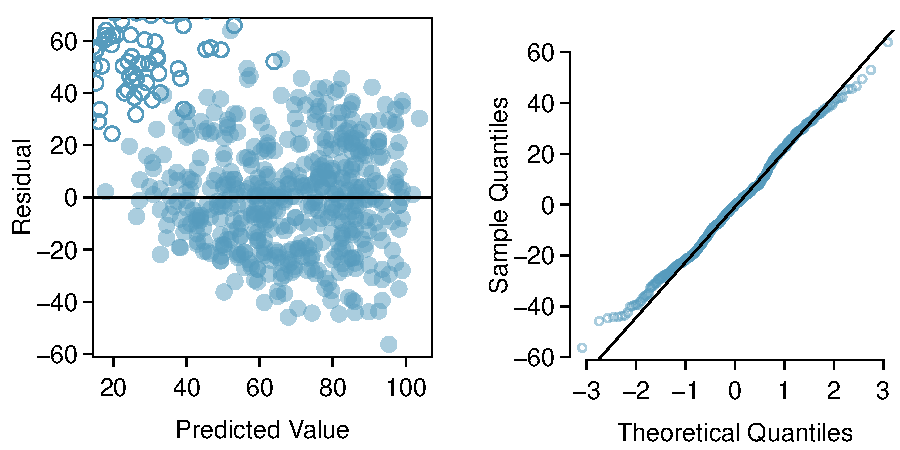
\includegraphics[width=0.8\textwidth]
	{ch_multiple_linear_regression_oi_biostat/figures/prevendRFFTStatinAgeEducCVDResidNormPlot/prevendRFFTStatinAgeEducCVDResidNormPlot.pdf}
	\caption{A histogram and normal probability plot of the residuals from the linear model for RFFT vs. statin use, age, educational level and presence of cardiovascular disease in the PREVEND data}
	\label{prevendRFFTStatinAgeEducCVDResidNormPlot}
\end{figure}

It is quite possible that even the model summarized in Table~\ref{prevendRFFTStatinAgeEducationCVD} is not the best one to understand the association of cognitive ability with statin use. There be other confounders that are not accounted for.  Possible predictors that may be confounders but have not been examined are called \term{residual confounders}.  Residual confounders can be other variables in a dataset that have not been examined, or variables that were not measured in the study.  Residual confounders exist in almost all observational studies, and represent one of the main reasons that observational studies should be interpreted with caution.  A randomized experiment is the best way to eliminate residual confounders. Randomization ensures that, at least on average, all predictors are not associated with the randomized intervention, which eliminates one of the conditions for confounding.  A randomized trial may be possible in some settings; there have been many randomized trials examining the effect of using statins. However, in many other settings, such as a study of the association of marijuana use and later addiction to controlled substances, randomization may not be possible or ethical.  In those instances, observational studies may be the best available approach.

\section{Interaction in regression}

An important assumption in the multiple regression model
\[y = \beta_0 + \beta_1x_1 + \beta_2x_2 + ... + \beta_px_p + \varepsilon \] 
is that when one of the variables changes (say, $x_j$) by 1 unit and all other variables do not change, the predicted response changes by $\beta_j$, regardless of the values of the other variables.  An statistical \term{interaction} occurs when this assumption is not true and the nature relationship of one explanatory variable $x_j$ with the response depends on the value of one or more other explanatory variables.

This is most easily understood in a model with two predictors,
Consider a model that might be used to predict total cholesterol level from age and diabetes status (either diabetic or non-diabetic).  
\[\text{TotChol} = \beta_0 + \beta_1\text{Age} + \beta_2\text{Diabetes} + \varepsilon \]
Assume that total cholesterol (\var{TotChol}) is measured in mmol/L, \var{Age} is recorded in years, and \var{Diabetes} is coded as 1 for a person with diabetes, and 0 otherwise.  For non-diabetics (\var{Diabetes} = 0), the linear relationship between cholesterol and age would be
\[TotChol = \beta_0 + \beta_1\text{Age} + \varepsilon. \]
The population regression line would have slope $\beta_1$ and intercept $\beta_0$.  For diabetics (\var{Diabetes} = 1), the population regression line becomes
\begin{align*}
\text{TotChol} &= \beta_0 + \beta_1\text{Age} + \beta_2 + \varepsilon \\
&= \beta_0 + \beta_2 + \beta_1\text{Age},
\end{align*}
a line with the same slope $\beta_1$ but different intercept $\beta_0 + \beta_2$.  The lines predicting cholesterol as a function of age in diabetics and non-diabetics are parallel lines with different intercept.  Cholesterol might be higher overall in diabetics than non-diabetics, but the changes in cholesterol as age changes will be the same in both groups.

Figure~\ref{modelNoInteraction} shows hypothetical  graphs of population regression lines in this setting when there is no statistical interaction between age and diabetes status.

% graphic needed here of parallel lines.  Might be a two panel plot, second panel showing interaction.

A relationship in which changes in cholesterol as a function of age does not depend on diabetes status might, however, be overly simple, and potentially misleading if it is wrong.

% begin example from nhanes here.



\section{Model selection and prediction}
\label{modelSelectionPrediction}

Forest birds

\section{The connection between ANOVA and regression}
\label{ANOVAandRegression}

Statins and education, refer to ch 5


\section{Notes}

This and the previous chapters have provided only an introduction to regression, with many advance topics not covered. But even this introduction provides useful tools for getting started on many analyses by following some commonly recommended steps.

\begin{itemize}
	
	\item Regression models are more reliable when the response variable has an approximate normal distribution, or at least a symmetric distribution.  Always begin by examining a histogram and normal probability plot of the response variable.  Right-skewed response variables are common, and a log transform will often produce approximate normality. The predictors need not be normally distributed; some may be categorical variables.  If a transformation is used for the response variable, the final interpretation of the any model should be stated in terms of the original scale of measurement for the response.
	
	\item When fitting a simple linear regression, make a scatterplot with a least squares line, even when the predictor is a categorical variable with two levels.  Nonlinear trends or outliers are often obvious in scatterplots.  If outliers are evident, the source of the data should when possible, since outliers result from errors in data collection.  If there has not been an error or the data collection process is not accessible, consider whether the outlier does not belong to the target population of inference, such as the District of Columbia in the data on infant mortality shown in Figure~\ref{infMortUS}.
	
	\item Keep a clear view of the purpose of the regression.  Will it be used to understand the relationship between a particular predictor and the response after adjusting for confounders, to construct a model for prediction, or to simply understand the joint association between a response and set of predictors.
	
	\item Building a model for prediction from a large set of potential predictors can be useful, but the best way to construct a multiple regression model is to think about the context of the problem and include predictors that have either been shown in the past to be associated with the response or for which there is a plausible working hypothesis about some association.
	
	\item When building a model where there may not be a clear specification of which predictors to include, it is useful to examine the association between the response and each of the individual predictors.  Remember that lack of statistical significance of the association between a response and a predictor is not evidence of no association, so predictors are often included in an initial model even when the evidence against no association is weaker than the traditional $p=0.05$.  In practice, investigators sometimes include predictors for which the individual associations are significant at $p < 0.10$ or $p < 0.20$.
	
	\item  With either simple or multiple regression, examine diagnostic plots of the residuals before drawing conclusions.  All models are approximations, and residual plots are seldom as perfectly behaved as in \data{statin.samp}, so don't fuss too much about relatively minor violations of the assumptions.  When the residual plots show some striking anomalies, as in the analysis of the \data{famuss} dataset, try to explore the anomalies for an explanation.  Even when they can't be `disappeared', it is useful to understand the source of the anomalies.
	
	\item  The summary statistics from a regression output, e.g., t-statistics, adjusted $R^2$ and $F$-statistics all provide different information and should be used appropriately.
	
	
	\begin{comment}
	multivariate definition of R-squared
	\end{comment}
\end{itemize}

To keep the treatment of regression both brief and accessible, however, many important topics have been left out.  Here are some of the most important

\begin{itemize}
	
	\item Predicted values from a regression have an inherent uncertainty because model parameters are only estimates.  There are two types of interval estimates used with prediction: confidence intervals for a predicted mean response from a set of values for the predictors; and prediction intervals that show the variability in predicted response for a set of predictors for a case not in the dataset.  Because prediction intervals are subject to both the variability in a predicted mean response and the variability of an individual observation about is mean, prediction intervals are wider than confidence intervals for a predicted mean.  Most statistical software provide both kinds of estimates.
	
	\item Model selection is a more advanced and more difficult topic that is often recognized by practitioners, and about which there is continuing research.  Many introductor texts recommend using `stepwise' regression.  Forward stepwise regression adds predictors one by one according to a set criterion (usually smallest $p$-value).  Backward stepwise regression eliminates variables from a larger model one by one until a criterion is met. Both approaches can be useful and usually automated in statistical software.  But there are weaknesses to both methods -- final models are data dependent and chance alone can lead to spurious variables being included.  Since the models are data-driven, traditional formulas for estimating prediction error underestimate the variability in predictions. In very large datasets, stepwise regression can lead to substantially incorrect models. Newer methods for model building based on cross-validation or other advanced techniques are more reliable.
	
	\item  Examining the significance levels of several regression coefficients involves (at least implicitly) testing several hypotheses simultaneously and can lead to increased type I error rate, of the sort discussed in Section~\ref{multipleComparisonsAndControllingTheType1ErrorRate}.  A less error-prone approach begins with the $F$statistic, and if it significant, adjusts $p$-value for multiplicity. For a small number of coefficients, a Bonferroni adjustment is useful, but more advanced methods of error control are used in datasets with more than a handful of parameters.  \textit{we are not following our own advice on this.}
	
\end{itemize}



\begin{comment}

- Add an data exercise showing that r-squared always increases but
that the adjusted r-squared 

- the section that introduces general multiple regression mentions
several applications of multiple regression (model selection, ANOVA)
but never illustrates those apps.  We should have a section on model
selection.  What about interaction in regression.

\end{comment}






